\chapter[Introduction]{Introduction}

\section{Motivation}

Humankind has only a few ways to generate reliable, nonintermittent 
base load power: fossil fuel, hydroelectric, geothermal, and 
nuclear energy. Because of increasing global warming and climate 
change concerns, sources that have negligible CO$_2$ footprints 
represent crucial measures for the control of global temperature change. 
From an environmental viewpoint, hydro and nuclear power are 
preferable ways to generate reliable power. Nevertheless, the 
potential for hydro power is strictly limited by local geographical 
conditions, hence, the only one option left is nuclear power. Nuclear 
power plants generate 4.9\% of global energy production \cite{noauthor_key_2017}, a figure which is projected to stay constant up to 2040 while 
electricity demand is predicted to increase by 30\% \cite{noauthor_world_2017}.  Unfortunately, because of concerns regarding safety, nuclear weapon 
proliferation, radioactive waste treatment, and competitiveness with 
other sources of energy (i.e. renewables), a negative public attitude 
to nuclear has formed in many developed countries, which makes it 
challenging to justify its zero emissions benefits.

\glsentryfirstplural{MSR} are among the six advanced reactor 
concepts that have been chosen by the Generation IV International 
Forum (GIF) for further research and development. \glspl{MSR} 
offer significant improvements ``in the four broad areas of 
sustainability, economics, safety and reliability, and proliferation 
resistance and physical protection" \cite{doe_technology_2002}. To 
achieve the goals formulated by the GIF, \glspl{MSR} attempt to 
simplify the reactor core and improve inherent safety by using 
liquid coolant which is also a fuel\footnote{Herein \glspl{MSR} are 
assumed to be reactors with liquid fuel which simultaneously serves 
as coolant.}. In a thermal spectrum \gls{MSR}, fluorides of fissile 
and/or fertile materials (i.e. UF$_4$, PuF$_3$ and/or ThF$_4$) are 
mixed with carrier salts to form a liquid fuel which is circulated 
in a loop-type primary circuit \cite{haubenreich_experience_1970}. 
This innovation leads to immediate advantages over traditional, 
solid-fueled, reactors. These include near-atmospheric pressure 
in the primary loop, relatively high coolant temperature, outstanding 
neutron economy, a high level of inherent safety, reduced fuel 
preprocessing, and the ability to continuously remove fission products 
and add fissile and/or fertile elements without shutdown  \cite{leblanc_molten_2010}. The possibility of continuously removing 
neutron poisons allows for a significant increase in fuel burnup and thus 
improves the resource utilization of \glspl{MSR}. Finally, the \gls{MSR} 
also could be employed as a converter reactor for transmutation of 
spent fuel from current \glspl{LWR}.

Recently, interest in \glspl{MSR} has resurged, with multiple new companies 
pursuing commercialization of \gls{MSR} designs\footnote{Examples 
include liquid-fueled molten salt designs from Terrapower, Terrestrial, 
ThorCon, Flibe, Copenhagen Atomics, etc.}. China's \gls{MSR} program 
was initiated in 2011 and promises to start-up a 2MW$_{th}$ 
liquid-fueled test \gls{MSR} (TMSR-LF1) in 2020, a 10MW$_{th}$ 
demonstration reactor (TMSR-LF2) in 2025, and a gigawatt-level 
commercial reactor in 2050 \cite{zhang_review_2018}. The European 
Union funds the Safety Assessment of the Molten Salt Fast Reactor 
(SAMOFAR) project, in which several European research institutes and 
universities are developing various molten salt reactor prototypes 
such as the \gls{MSFR} \cite{fiorina_molten_2013} and the \gls{MOSART} 
\cite{ignatiev_molten_2014}.
To further develop these \gls{MSR} concepts, particularly with respect 
to their strategies for online reprocessing and refueling, 
computational analysis methods capturing their unique reactor physics 
and process chemistry are needed.

However, most contemporary nuclear reactor physics software is unable 
to perform depletion calculations in an online reprocessing regime. 
To correctly determine properties and operation of \glspl{MSR}, 
including injection/removal schemes, computational tools to accurately 
model the processes which are unique for this particular reactor type. Specifically, the circulation of the liquid fuel and the continuous 
feed or removal of elements (e.g. fissile material injection into 
and \glspl{FP} extraction from the fuel salt) are put-of-scope for 
most contemporary nuclear reactor physics software, which were 
originally written primarily to simulate solid-fuel reactors. 
Thus, a numerical simulation package that would be able to model 
nuclear reactors with circulating fuel is needed to close the gap.

\section{Methodology}
The main objective of proposed work is developing the online 
reprocessing simulation package, SaltProc, which expands the 
capability of the continuous-energy Monte Carlo depletion 
calculation code, SERPENT2 \cite{leppanen_serpent_2015}, for 
liquid-fueled \glspl{MSR} simulations. The SaltProc package 
will enable the simulation of neutron poisons extraction 
based on physics- and chemistry-driven correlations. 
Moreover, it will take into account the non-instantaneous 
nature of injection/removal processes and material decay. 
The ultimate objective of this effort is to develop a generic 
open-source tool capable of simulate a wide range of 
liquid-fueled systems including two-fluid and multi-region 
designs, and validate it against existing modeling efforts. 
Figure~\ref{fig:workflow_method} illustrates my previous 
research effort and the proposed plan towards the objective 
described above.
\begin{figure}[htp!] % replace 't' with 'b' to 
  \centering
	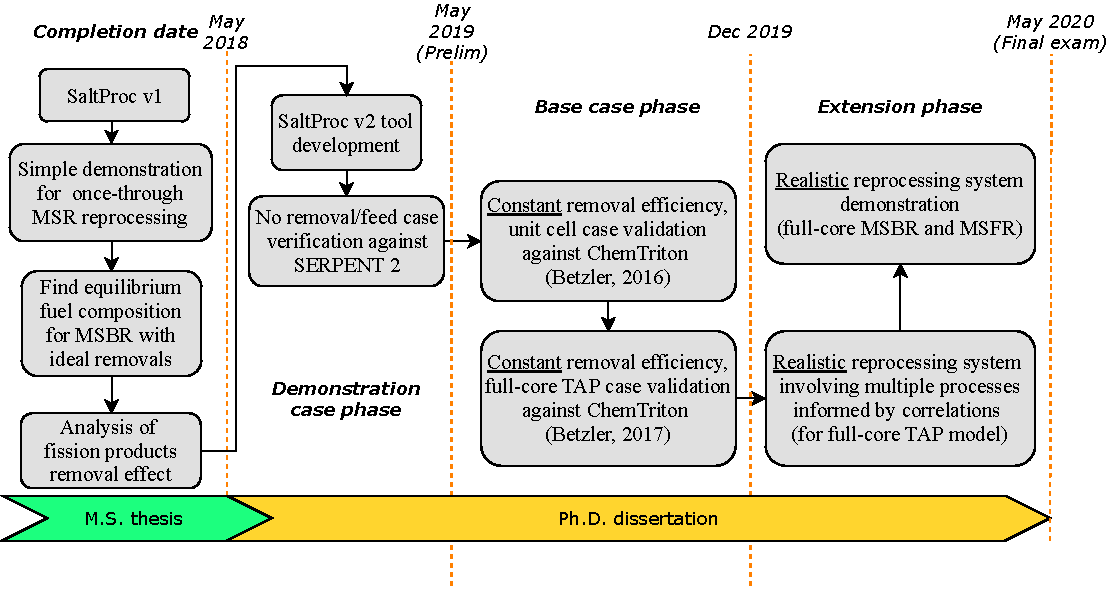
\includegraphics[width=\textwidth]{workflow_for_methodology.pdf}
  \caption{Workflow for completed (M.Sc. thesis) and proposed (Ph.D.) work 
  which includes the tool demonstration and validation for the \gls{TAP} 
  reactor, the \gls{MSBR}, and the \gls{MSFR}.}
  \label{fig:workflow_method}
\end{figure}

In this work current published online reprocessing simulation efforts 
have been systematized, investigated and reviewed to identify desirable 
generic reprocessing code capabilities. A preliminary set of key input 
and output parameters, software package architecture and class 
structure, and required capabilities has been chosen to conceptually 
capture the fundamental online reprocessing challenges. 

Three perspective liquid-fueled \gls{MSR} concepts among various 
fuel cycles, number of salts (single- and two-fluid), neutron 
spectra and reprocessing schemes will be investigated to 
demonstrate and validate proposed simulation package. Specifically, 
the demonstration and validation efforts will be focused on the \gls{TAP} 
\gls{MSR} which is relatively well described in the literature. 
The results obtained with SaltProc will be verified against 
recent online reprocessing efforts in the literature for the 
\gls{TAP} reactor, the \gls{MSBR}, and the \gls{MSFR}. 